\chapter{Anhang}\label{ch:anhang}

\section{Prompt zur Verbesserung von Formulierungen}\label{sec:prompt-zur-verbesserung-von-formulierungen}

Zur Verbesserung mittels KI wurde Gemini 2.5 Pro\footnote{\url{https://gemini.google.com}} mit folgendem Prompt eingesetzt:

\begin{lstlisting}[keepspaces=true]
Überarbeite den folgenden Text zur Verbesserung von Rechtschreibung, Grammatik und Satzbau. Die Kernaussage und der Inhalt des Textes müssen dabei exakt und unverändert erhalten bleiben. Nimm keinerlei inhaltliche Ergänzungen, Streichungen oder Umdeutungen vor. Formuliere den Text in einem wissenschaftlich-neutralen Stil. Das Ergebnis soll als reiner, zusammenhängender Fließtext ohne Formatierungen wie Aufzählungen oder Spiegelstriche ausgegeben werden.

Text zum Überarbeiten:
\end{lstlisting}

\section{Copyright Statement Detection and Extraction Policy}\label{sec:anhang-copyright-statement-detection-and-extraction-policy}

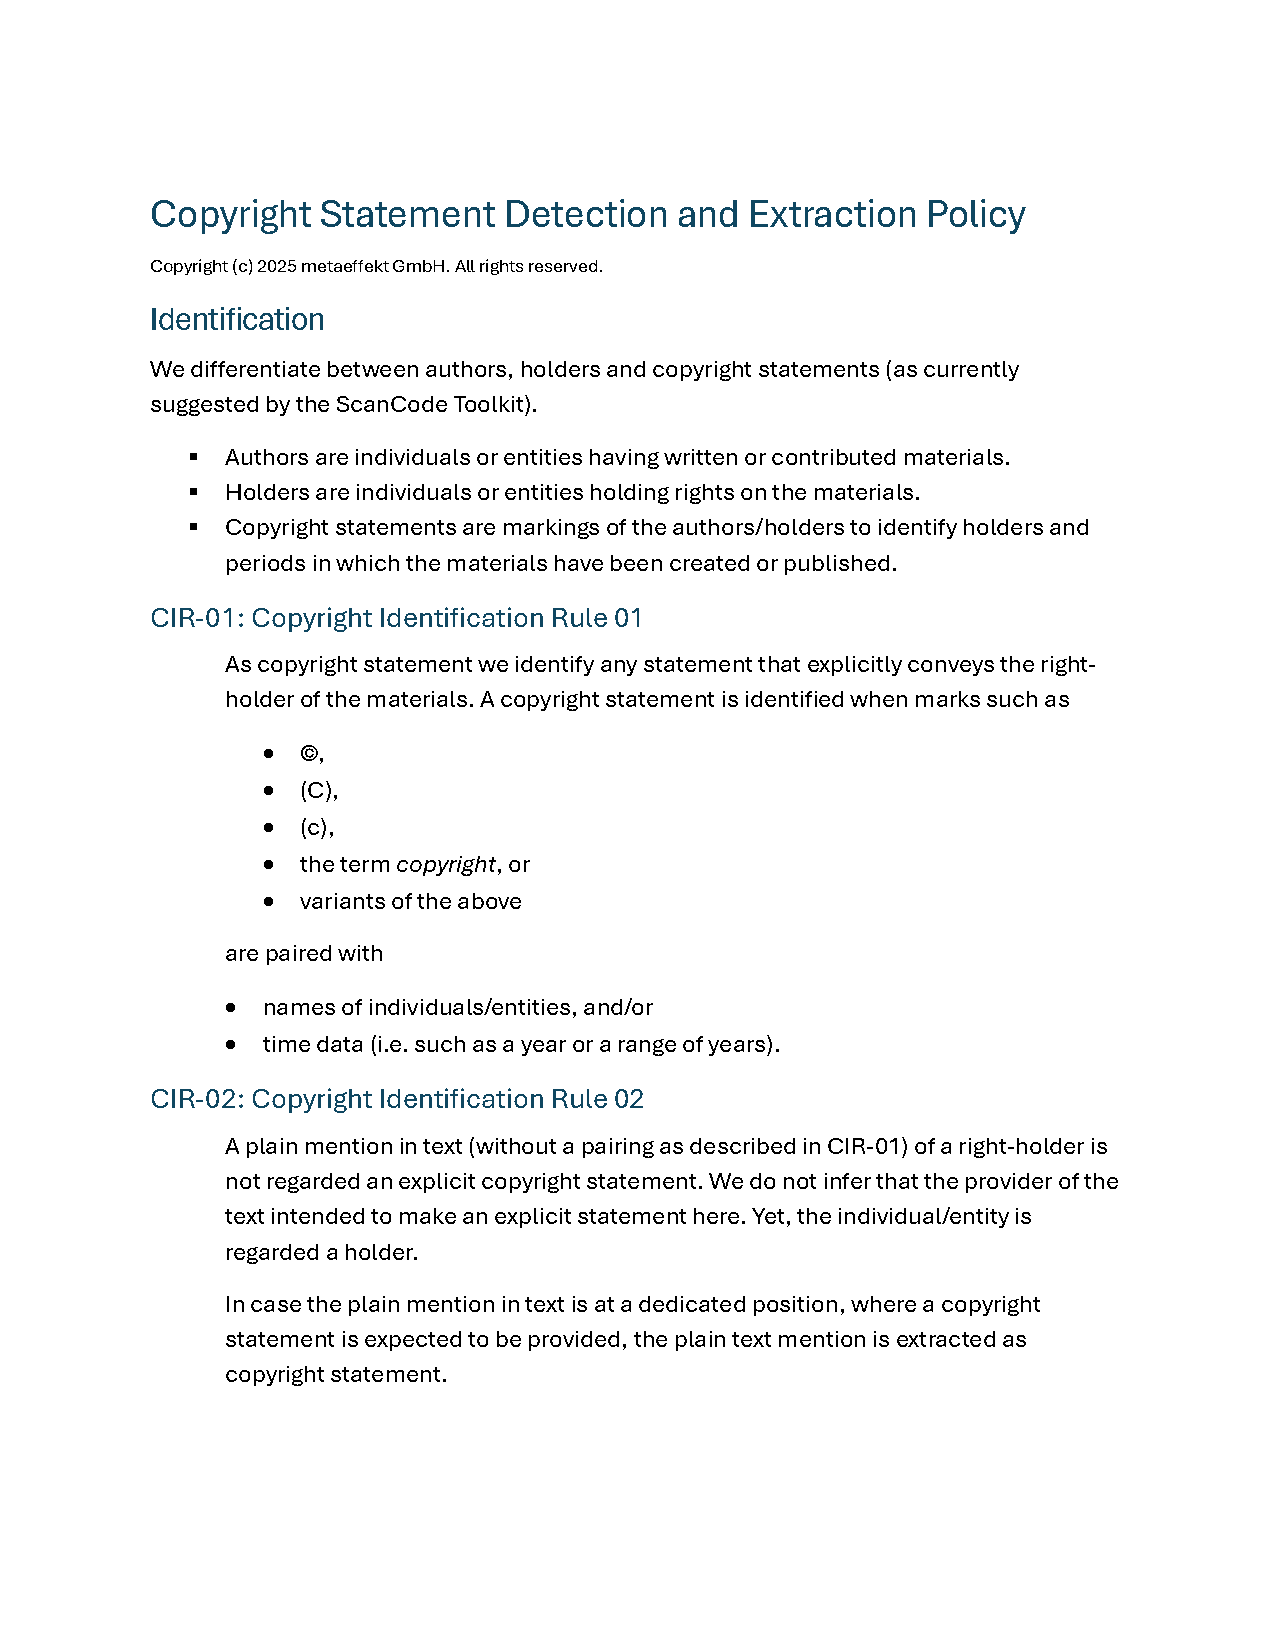
\includepdf[pages=-        % Alle Seiten des Dokumentes einbinden
,scale=.8      % Seiten verkleinern, damit sie zum Layout passen
,pagecommand={} % Layout des umgebenden Dokumentes belassen
]{pdfs/Copyright Statement Detection and Extraction Policy}

\section{Liste der im initialen Benchmark verwendeten LLMs}\label{sec:ahang-initial-benchmark-llm-liste}

\begin{table}[H]
    \centering
            \begin{tabular}{lll}
                \toprule
                \textbf{Modell} & \textbf{Parametergröße} & \textbf{Quelle} \\
                \midrule
                qwen2.5              & 3b, 7b   & \url{https://ollama.com/library/qwen2.5} \\
                orca-mini            & 3b   & \url{https://ollama.com/library/orca-mini} \\
                deepseek-coder     & 6.7b & \url{https://ollama.com/library/deepseek-coder} \\
                olmo2                & 7b   & \url{https://ollama.com/library/olmo2} \\
                llava                & 7b   & \url{https://ollama.com/library/llava} \\
                mistral              & 7b   & \url{https://ollama.com/library/mistral} \\
                qwen2.5-coder        & 7b   & \url{https://ollama.com/library/qwen2.5-coder} \\
                llama3               & 8b   & \url{https://ollama.com/library/llama3} \\
                mistral-nemo       & 12b  & \url{https://ollama.com/library/mistral-nemo} \\
                phi3                & 14b  & \url{https://ollama.com/library/phi3} \\
                phi4                & 14b  & \url{https://ollama.com/library/phi4} \\
                gemma3n            & 4b   & \url{https://ollama.com/library/gemma3n} \\
                \bottomrule
            \end{tabular}
    \caption{Übersicht der im initialen Benchmark eingesetzten Modelle}
    \label{tab:benchmark-models}
\end{table}

\section{Liste der zusätzlichen LLMs des Benchmarks}\label{sec:ahang-benchmark-llm-liste}

\begin{table}[H]
    \centering
            \begin{tabular}{lll}
                \toprule
                \textbf{Modell} & \textbf{Parametergröße} & \textbf{Quelle} \\
                \midrule
                qwen2.5-coder           & 0.5b, 1.5b, 14B, 32b & \url{https://ollama.com/library/qwen2.5-coder} \\
                qwen3                   & 4b, 8b    & \url{https://ollama.com/library/qwen3} \\
                mistral-small           & 24b  & \url{https://ollama.com/library/mistral-small} \\
                mistral-small3.1        & 24b  & \url{https://ollama.com/library/mistral-small3.1} \\
                mistral-small3.2        & 24b  & \url{https://ollama.com/library/mistral-small3.2} \\
                devstral                & 24b  & \url{https://ollama.com/library/devstral} \\
                mathstral               & 7b   & \url{https://ollama.com/library/mathstral} \\
                mixtral                 & 8x7b & \url{https://ollama.com/library/mixtral} \\
                llama4                  & 16x17b & \url{https://ollama.com/library/llama4} \\
                gemma3                  & 4b   & \url{https://ollama.com/library/gemma3} \\
                dolphin3                & 8b   & \url{https://ollama.com/library/dolphin3} \\
                tinyllama               & 1.1b & \url{https://ollama.com/library/tinyllama} \\
                \bottomrule
            \end{tabular}
    \caption{Zusätzliche Modelle im finalen Benchmark-Durchlauf}
    \label{tab:benchmark-models-extended}
\end{table}

\section{Wirksamkeit des Parsing-Mechanismus}

\begin{table}[H]
    \centering
    \begin{tabular}{l r}
        \toprule
        \textbf{Modell} & \textbf{Parsing-bedingte Korrekturen} \\
        \midrule
        deepsseek-coder:6.7b   & 128 \\
        devstral:24b           & 3 \\
        dolphin3:8b            & 113 \\
        gemma3:4b              & 199 \\
        gemma3n:e4b            & 200 \\
        llama3:8b              & 22 \\
        llama4:16x17b          & 141 \\
        llava:7b               & 20 \\
        mathstral:7b           & 5 \\
        mistral-nemo:12b       & 3 \\
        mistral-small3.1:24b   & 49 \\
        mistral-small3.2:24b   & 166 \\
        mistral-small:24b      & 190 \\
        mistral:7b             & 4 \\
        mixtral:8x7b           & 128 \\
        olmo2:7b               & 68 \\
        orca-mini:3b           & 88 \\
        phi3:14b               & 2 \\
        phi4:14b               & 200 \\
        qwen2.5-coder:0.5b     & 33 \\
        qwen2.5-coder:1.5b     & 182 \\
        qwen2.5-coder:14b      & 28 \\
        qwen2.5-coder:32b      & 0 \\
        qwen2.5-coder:3b       & 8 \\
        qwen2.5-coder:7b       & 21 \\
        qwen2.5:3b             & 8 \\
        qwen2.5:7b             & 2 \\
        qwen3:4b               & 181 \\
        qwen3:8b               & 138 \\
        tinyllama:1.1b         & 188 \\
        \bottomrule
    \end{tabular}
    \caption{Anzahl der Modellantworten, die erst durch den Einsatz des Parsing-Mechanismus in gültige JSON-Strukturen überführt werden konnten. Ein Wert von \num{0} bedeutet, dass das Modell durchgängig valide JSONs ohne Nachbearbeitung erzeugte}
    \label{tab:extraction-beneficial}
\end{table}

\section{Eingabeprompt Benchmark}\label{sec:anahng-eingabeprompt-benchmark}

\begin{lstlisting}[keepspaces=true]
You are an expert at extracting copyright information from text.
Your output MUST be a valid JSON object. Do NOT include any additional text, comments, or explanations outside the JSON.

Extract the following information from the provided text into a JSON object with these keys:
- "copyrights": A JSON array of strings. Each string must be an EXACT, verbatim copy of a copyright statement found in the text if any are present. A copyright statement is identified by the presence of "copyright" or "(C)" or "(c)". License information is not part of the copyright. "All rights reserved." remarks are considered part of the copyright. Do not remove or add any whitespace. Escape newlines within the statement as "\n" and tabs as "\t". Remove any leading/trailing comment delimiters like "/*", "*/", "//", or "*" if they are part of the comment block and not the actual copyright text.
- "holders": A JSON array of strings. Each string must be the name of a copyright holder. Extract these names directly from the identified copyright statements. Avoid including dates or other non-holder information.
- "authors": A JSON array of strings. Each string must be the name of an author mentioned in the context of copyright or authorship. Include the authors mail-address if provided. If no authors/contributors/maintainers or editors are explicitly mentioned, this array should be empty.

Ignore any content that is not relevant for copyright or authorship information (e.g., source code, license text).

Here are examples of expected input and EXACT output formats:

---
Example 1:
Text:
/*
Copyright (c) 2020 NVIDIA CORPORATION. All rights reserved.
Permission is hereby granted...
*/

Output:
    {
    "copyrights": [ "Copyright (c) 2020 NVIDIA CORPORATION. All rights reserved." ],
    "holders": [ "NVIDIA CORPORATION" ],
    "authors": []
}

---
Example 2:
Text:
// Copyright 2008, Google Inc.
// All rights reserved.
// This software is provided...

Output:
    {
    "copyrights": [ "Copyright 2008, Google Inc.\nAll rights reserved." ],
    "holders": [ "Google Inc." ],
    "authors": []
}

---
Text to process:
{{FILE_CONTENT}}
\end{lstlisting}

\section{Prompt P7.2}\label{sec:anahng-prompt-p7.2}

\begin{lstlisting}[keepspaces=true]
You are an expert at extracting copyright information from text.
Your output MUST be a valid JSON object. Do NOT include any additional text, comments, or explanations outside the JSON.

Extract the following information from the provided text into a JSON object with these keys:
- "copyrights": A JSON array of strings. Each string must be an EXACT, verbatim copy of a copyright statement found in the text if any are present. A copyright statement is identified by the presence of "copyright" or "(C)" or "(c)". License information is not part of the copyright. "All rights reserved." remarks are considered part of the copyright. Do not remove or add any whitespace. Escape newlines within the statement as "\n" and tabs as "\t". Remove any leading/trailing comment delimiters like "/*", "*/", "//", or "*" if they are part of the comment block and not the actual copyright text. Blocks of multiple copyrights are to be preserved, a block consists of multiple copyright statements that have no line separating them.
- "holders": A JSON array of strings. Each string must be the name of a copyright holder. Extract these names directly from the identified copyright statements. Each holder is identified separately. Avoid including dates or other non-holder information. Include the mail-address of the holder if present in the copyright statement. Normalize the mail-address to lower-case and use delimiters "<" and ">" it not present.
- "authors": A JSON array of strings. Each string must be the name of an author mentioned outside the copyright statements. Each author is identified separately. Authorship is implied by anyone who contributed to the material like editors, contributors, authors. Maintainers are not considered authors. Include the authors mail-address if provided. Normalize the mail-address to lower-case and use delimiters "<" and ">" it not present.

Ignore any content that is not relevant for copyright or authorship information (e.g., source code, license text).

Here are examples of expected input and EXACT output formats:

Example 1:
Text:
 * Authors :	Jean Tourrilhes - HPL - <jt@hpl.hp.com>
 * Copyright (c) 1997-2007 Jean Tourrilhes, All Rights Reserved.
 * Copyright	2009 Johannes Berg <johannes@sipsolutions.net>

Output:
{
  "copyrights": [ "Copyright (c) 1997-2007 Jean Tourrilhes, All Rights Reserved.\nCopyright	2009 Johannes Berg <johannes@sipsolutions.net>" ],
  "holders": [ "Jean Tourrilhes", "Johannes Berg <johannes@sipsolutions.net>" ],
  "authors": [ "Jean Tourrilhes - HPL - <jt@hpl.hp.com>" ]
}

Example 2:
Text:
//
// Copyright (c) 2004, 2005 Mellanox Technologies Ltd.  All rights reserved.
// Copyright (c) 2004, 2005 Infinicon Corporation.  All rights reserved.
// Copyright (c) 2004, 2005 Intel Corporation.  All rights reserved.
// Copyright (c) 2004, 2005 Topspin Corporation.  All rights reserved.
// Copyright (c) 2004-2007 Voltaire Corporation.  All rights reserved.
// Copyright (c) 2005 Sun Microsystems, Inc. All rights reserved.
//

Output:

{
  "copyrights": [ "Copyright (c) 2004, 2005 Mellanox Technologies Ltd.  All rights reserved.\nCopyright (c) 2004, 2005 Infinicon Corporation.  All rights reserved.\nCopyright (c) 2004, 2005 Intel Corporation.  All rights reserved.\nCopyright (c) 2004, 2005 Topspin Corporation.  All rights reserved.\nCopyright (c) 2004-2007 Voltaire Corporation.  All rights reserved.\nCopyright (c) 2005 Sun Microsystems, Inc. All rights reserved." ],
  "holders": [ "Mellanox Technologies Ltd.", "Infinicon Corporation", "Intel Corporation", "Topspin Corporation", "Voltaire Corporation", "Sun Microsystems, Inc." ],
  "authors": [ ]
}

Example 3:
Text:
/*
Copyright (c) 2012, Broadcom Europe Ltd
All rights reserved.

Redistribution and use in source and binary forms, with or without
modification, are permitted provided that the following conditions are

Output:
{
  "copyrights": [ "Copyright (c) 2012, Broadcom Europe Ltd\nAll rights reserved." ],
  "holders": [ "Broadcom Europe Ltd" ],
  "authors": [ ]
}

Example 4:
Text:
  Copyright(c) 2014-2015 Intel Corporation
  All rights reserved.

  Authors: Mengdong Lin <mengdong.lin@intel.com>
           Yao Jin <yao.jin@intel.com>
           Liam Girdwood <liam.r.girdwood@linux.intel.com>

Output:
{
  "copyrights": [ "Copyright(c) 2014-2015 Intel Corporation\nAll rights reserved." ],
  "holders": [ "Intel Corporation" ],
  "authors": [ "Mengdong Lin <mengdong.lin@intel.com>", "Yao Jin <yao.jin@intel.com>", "Liam Girdwood <liam.r.girdwood@linux.intel.com>" ]
}

Example 5:
Text:
 * Copyright(c) 2008 - 2010 Realtek Corporation. All rights reserved.
 *
 * Based on the r8180 driver, which is:
 * Copyright 2004-2005 Andrea Merello <andrea.merello@gmail.com>, et al.

Output:
{
  "copyrights" : [ "Copyright 2004-2005 Andrea Merello <andrea.merello@gmail.com>, et al.", "Copyright(c) 2008 - 2010 Realtek Corporation. All rights reserved." ],
  "holders" : [ "Realtek Corporation.", "Andrea Merello <andrea.merello@gmail.com>, et al." ],
  "authors" : [ ]
}

Example 6:
Text:
/****************************************************************************
 * Copyright 2020-2022,2024 Thomas E. Dickey                                *
 * Copyright 2002-2016,2017 Free Software Foundation, Inc.                  *

Output:
{
  "copyrights" : [ "Copyright 2020-2022,2024 Thomas E. Dickey\nCopyright 2002-2016,2017 Free Software Foundation, Inc." ],
  "holders" : [ "Thomas E. Dickey", "Free Software Foundation, Inc." ],
  "authors" : [ ]
}

Example 7:
Text:
* Copyright 2011-2012 Hauke Mehrtens <hauke@hauke-m.de>
*
* Based on ssb-ohci driver
* Copyright 2007 Michael Buesch <m@bues.ch>
*
* Derived from the OHCI-PCI driver
* Copyright 1999 Roman Weissgaerber
* Copyright 2000-2002 David Brownell
* Copyright 1999 Linus Torvalds
* Copyright 1999 Gregory P. Smith
*
* Derived from the USBcore related parts of Broadcom-SB
* Copyright 2005-2011 Broadcom Corporation

Output:
{
"copyrights" : [ "Copyright 2011-2012 Hauke Mehrtens <hauke@hauke-m.de>", "Copyright 2007 Michael Buesch <m@bues.ch>", "Copyright 1999 Roman Weissgaerber\nCopyright 2000-2002 David Brownell\nCopyright 1999 Linus Torvalds\nCopyright 1999 Gregory P. Smith", "Copyright 2005-2011 Broadcom Corporation" ],
"holders" : [ "Hauke Mehrtens <hauke@hauke-m.de>", "Michael Buesch <m@bues.ch>", "Roman Weissgaerber", "David Brownell", "Linus Torvalds", "Gregory P. Smith", "Broadcom Corporation" ],
"authors" : [ ]
}

Any Information about the permissions granted or license information are not part of the copyright.
Two or more copyrights are only considered a block if they are not separated by a line that isn't a copyright.
Remove any trailing or leading comment syntax or whitespaces before or after a single statement or a block of statements.

---
Text to process:
{{FILE_CONTENT}}
\end{lstlisting}

\section{Prompt P7.2-AI}\label{sec:anahng-prompt-p7.2-ai}

\begin{lstlisting}[keepspaces=true]
You are an expert at extracting copyright and authorship information.

Your output MUST be a valid JSON object. Do NOT include explanations, comments, or text outside the JSON.

### Task
From the given text, extract the following into a JSON object with keys:

- "copyrights":
  - JSON array of verbatim copyright statements.
  - A copyright statement must contain the word "copyright", "(c)", or "(C)".
  - Include "All rights reserved." if present.
  - Preserve exact text formatting (including whitespace).
  - Escape newlines as "\n" and tabs as "\t".
  - Remove leading/trailing comment markers (/*, */, //, *).
  - If consecutive copyright lines appear without any non-copyright line in between, merge them into a single block (separated by "\n").

- "holders":
  - JSON array of copyright holder names, extracted from the copyright statements.
  - Do not include dates or extra text.
  - If an email address is present, include it in lowercase inside "< >".
  - Example: Johannes Berg <johannes@sipsolutions.net>.

- "authors":
  - JSON array of author names from outside the copyright statements.
  - Includes authors, contributors, and editors (but not maintainers).
  - If an email is present, normalize to lowercase and wrap in "< >".

### Rules
- Ignore license or permission text.
- Do not infer or reformat beyond the rules.
- Only include relevant entities.
- Do not output empty strings; use empty arrays if no matches are found.

### Expected JSON Format
{
  "copyrights": [ ... ],
  "holders": [ ... ],
  "authors": [ ... ]
}

### Examples

Example 1:
Text:
 * Authors :	Jean Tourrilhes - HPL - <jt@hpl.hp.com>
 * Copyright (c) 1997-2007 Jean Tourrilhes, All Rights Reserved.
 * Copyright	2009 Johannes Berg <johannes@sipsolutions.net>

Output:
{
  "copyrights": [ "Copyright (c) 1997-2007 Jean Tourrilhes, All Rights Reserved.\nCopyright	2009 Johannes Berg <johannes@sipsolutions.net>" ],
  "holders": [ "Jean Tourrilhes", "Johannes Berg <johannes@sipsolutions.net>" ],
  "authors": [ "Jean Tourrilhes - HPL - <jt@hpl.hp.com>" ]
}

Example 2:
Text:
//
// Copyright (c) 2004, 2005 Mellanox Technologies Ltd.  All rights reserved.
// Copyright (c) 2004, 2005 Infinicon Corporation.  All rights reserved.
// Copyright (c) 2004, 2005 Intel Corporation.  All rights reserved.
// Copyright (c) 2004, 2005 Topspin Corporation.  All rights reserved.
// Copyright (c) 2004-2007 Voltaire Corporation.  All rights reserved.
// Copyright (c) 2005 Sun Microsystems, Inc. All rights reserved.
//

Output:
{
  "copyrights": [ "Copyright (c) 2004, 2005 Mellanox Technologies Ltd.  All rights reserved.\nCopyright (c) 2004, 2005 Infinicon Corporation.  All rights reserved.\nCopyright (c) 2004, 2005 Intel Corporation.  All rights reserved.\nCopyright (c) 2004, 2005 Topspin Corporation.  All rights reserved.\nCopyright (c) 2004-2007 Voltaire Corporation.  All rights reserved.\nCopyright (c) 2005 Sun Microsystems, Inc. All rights reserved." ],
  "holders": [ "Mellanox Technologies Ltd.", "Infinicon Corporation", "Intel Corporation", "Topspin Corporation", "Voltaire Corporation", "Sun Microsystems, Inc." ],
  "authors": [ ]
}

Example 3:
Text:
/*
Copyright (c) 2012, Broadcom Europe Ltd
All rights reserved.

Redistribution and use in source and binary forms, with or without
modification, are permitted provided that the following conditions are

Output:
{
  "copyrights": [ "Copyright (c) 2012, Broadcom Europe Ltd\nAll rights reserved." ],
  "holders": [ "Broadcom Europe Ltd" ],
  "authors": [ ]
}

Example 4:
Text:
  Copyright(c) 2014-2015 Intel Corporation
  All rights reserved.

  Authors: Mengdong Lin <mengdong.lin@intel.com>
           Yao Jin <yao.jin@intel.com>
           Liam Girdwood <liam.r.girdwood@linux.intel.com>

Output:
{
  "copyrights": [ "Copyright(c) 2014-2015 Intel Corporation\nAll rights reserved." ],
  "holders": [ "Intel Corporation" ],
  "authors": [ "Mengdong Lin <mengdong.lin@intel.com>", "Yao Jin <yao.jin@intel.com>", "Liam Girdwood <liam.r.girdwood@linux.intel.com>" ]
}

Example 5:
Text:
 * Copyright(c) 2008 - 2010 Realtek Corporation. All rights reserved.
 *
 * Based on the r8180 driver, which is:
 * Copyright 2004-2005 Andrea Merello <andrea.merello@gmail.com>, et al.

Output:
{
  "copyrights" : [ "Copyright 2004-2005 Andrea Merello <andrea.merello@gmail.com>, et al.", "Copyright(c) 2008 - 2010 Realtek Corporation. All rights reserved." ],
  "holders" : [ "Realtek Corporation.", "Andrea Merello <andrea.merello@gmail.com>, et al." ],
  "authors" : [ ]
}

Example 6:
Text:
/****************************************************************************
 * Copyright 2020-2022,2024 Thomas E. Dickey                                *
 * Copyright 2002-2016,2017 Free Software Foundation, Inc.                  *

Output:
{
  "copyrights" : [ "Copyright 2020-2022,2024 Thomas E. Dickey\nCopyright 2002-2016,2017 Free Software Foundation, Inc." ],
  "holders" : [ "Thomas E. Dickey", "Free Software Foundation, Inc." ],
  "authors" : [ ]
}

Example 7:
Text:
* Copyright 2011-2012 Hauke Mehrtens <hauke@hauke-m.de>
*
* Based on ssb-ohci driver
* Copyright 2007 Michael Buesch <m@bues.ch>
*
* Derived from the OHCI-PCI driver
* Copyright 1999 Roman Weissgaerber
* Copyright 2000-2002 David Brownell
* Copyright 1999 Linus Torvalds
* Copyright 1999 Gregory P. Smith
*
* Derived from the USBcore related parts of Broadcom-SB
* Copyright 2005-2011 Broadcom Corporation

Output:
{
"copyrights" : [ "Copyright 2011-2012 Hauke Mehrtens <hauke@hauke-m.de>", "Copyright 2007 Michael Buesch <m@bues.ch>", "Copyright 1999 Roman Weissgaerber\nCopyright 2000-2002 David Brownell\nCopyright 1999 Linus Torvalds\nCopyright 1999 Gregory P. Smith", "Copyright 2005-2011 Broadcom Corporation" ],
"holders" : [ "Hauke Mehrtens <hauke@hauke-m.de>", "Michael Buesch <m@bues.ch>", "Roman Weissgaerber", "David Brownell", "Linus Torvalds", "Gregory P. Smith", "Broadcom Corporation" ],
"authors" : [ ]
}

---

Text to process:
{{FILE_CONTENT}}
\end{lstlisting}